% This file was converted to LaTeX by Writer2LaTeX ver. 1.0.2
% see http://writer2latex.sourceforge.net for more info
\documentclass{tufte-book}

\usepackage[utf8]{inputenc}
\usepackage[T1]{fontenc}
\usepackage[spanish]{babel}
\usepackage{amsmath}
\usepackage{amssymb,amsfonts,textcomp}
\usepackage{array}
\usepackage{supertabular}
\usepackage{hhline}
\usepackage{graphicx}

\makeatletter
\newcommand\arraybslash{\let\\\@arraycr}
\makeatother
\setlength\tabcolsep{1mm}
\renewcommand\arraystretch{1.3}
\newcommand\wideslash[2]{{}^{#1}/_{#2}}
\newcommand\normalsubformula[1]{\text{\mathversion{normal}$#1$}}
\title{I - INTRODUCCIÓN:}
\author{SOL}
\date{2011-09-01}

\hypersetup{colorlinks}% uncomment this line if you prefer colored hyperlinks (e.g., for onscreen viewing)

%%
% Book metadata
\title{Representaciónes \\ Cartográficas \thanks{Thanks to Edward R.~Tufte for his inspiration.}}
\author[Miguel Starobinsky \ Javier Clavijo]{Miguel Starobinsky \ Javier Clavijo}
\publisher{Publisher of This Book}

%%
% If they're installed, use Bergamo and Chantilly from www.fontsite.com.
% They're clones of Bembo and Gill Sans, respectively.
%\IfFileExists{bergamo.sty}{\usepackage[osf]{bergamo}}{}% Bembo
%\IfFileExists{chantill.sty}{\usepackage{chantill}}{}% Gill Sans

%\usepackage{microtype}

%%
% Just some sample text
\usepackage{lipsum}

%%
% For nicely typeset tabular material
\usepackage{booktabs}

%%
% For graphics / images
\usepackage{graphicx}
\setkeys{Gin}{width=\linewidth,totalheight=\textheight,keepaspectratio}
\graphicspath{{graphics/}}

% The fancyvrb package lets us customize the formatting of verbatim
% environments.  We use a slightly smaller font.
\usepackage{fancyvrb}
\fvset{fontsize=\normalsize}

%%
% Prints argument within hanging parentheses (i.e., parentheses that take
% up no horizontal space).  Useful in tabular environments.
\newcommand{\hangp}[1]{\makebox[0pt][r]{(}#1\makebox[0pt][l]{)}}

%%
% Prints an asterisk that takes up no horizontal space.
% Useful in tabular environments.
\newcommand{\hangstar}{\makebox[0pt][l]{*}}

%%
% Prints a trailing space in a smart way.
\usepackage{xspace}

%%
% Some shortcuts for Tufte's book titles.  The lowercase commands will
% produce the initials of the book title in italics.  The all-caps commands
% will print out the full title of the book in italics.
\newcommand{\vdqi}{\textit{VDQI}\xspace}
\newcommand{\ei}{\textit{EI}\xspace}
\newcommand{\ve}{\textit{VE}\xspace}
\newcommand{\be}{\textit{BE}\xspace}
\newcommand{\VDQI}{\textit{The Visual Display of Quantitative Information}\xspace}
\newcommand{\EI}{\textit{Envisioning Information}\xspace}
\newcommand{\VE}{\textit{Visual Explanations}\xspace}
\newcommand{\BE}{\textit{Beautiful Evidence}\xspace}

\newcommand{\TL}{Tufte-\LaTeX\xspace}

% Prints the month name (e.g., January) and the year (e.g., 2008)
\newcommand{\monthyear}{%
  \ifcase\month\or Enero\or Febrero\or Marzo\or Abril\or Mayo\or Junio\or
  Julio\or Agosto\or Septiembre\or Octubre\or Noviembre\or
  Diciembre\fi\space\number\year
}


% Prints an epigraph and speaker in sans serif, all-caps type.
\newcommand{\openepigraph}[2]{%
  %\sffamily\fontsize{14}{16}\selectfont
  \begin{fullwidth}
  \sffamily\large
  \begin{doublespace}
  \noindent\allcaps{#1}\\% epigraph
  \noindent\allcaps{#2}% author
  \end{doublespace}
  \end{fullwidth}
}

% Inserts a blank page
\newcommand{\blankpage}{\newpage\hbox{}\thispagestyle{empty}\newpage}

\usepackage{units}

% Typesets the font size, leading, and measure in the form of 10/12x26 pc.
\newcommand{\measure}[3]{#1/#2$\times$\unit[#3]{pc}}

% Macros for typesetting the documentation
\newcommand{\hlred}[1]{\textcolor{Maroon}{#1}}% prints in red
\newcommand{\hangleft}[1]{\makebox[0pt][r]{#1}}
\newcommand{\hairsp}{\hspace{1pt}}% hair space
\newcommand{\hquad}{\hskip0.5em\relax}% half quad space
\newcommand{\TODO}{\textcolor{red}{\bf TODO!}\xspace}
\newcommand{\na}{\quad--}% used in tables for N/A cells
\providecommand{\XeLaTeX}{X\lower.5ex\hbox{\kern-0.15em\reflectbox{E}}\kern-0.1em\LaTeX}
\newcommand{\tXeLaTeX}{\XeLaTeX\index{XeLaTeX@\protect\XeLaTeX}}
% \index{\texttt{\textbackslash xyz}@\hangleft{\texttt{\textbackslash}}\texttt{xyz}}
\newcommand{\tuftebs}{\symbol{'134}}% a backslash in tt type in OT1/T1
\newcommand{\doccmdnoindex}[2][]{\texttt{\tuftebs#2}}% command name -- adds backslash automatically (and doesn't add cmd to the index)
\newcommand{\doccmddef}[2][]{%
  \hlred{\texttt{\tuftebs#2}}\label{cmd:#2}%
  \ifthenelse{\isempty{#1}}%
    {% add the command to the index
      \index{#2 command@\protect\hangleft{\texttt{\tuftebs}}\texttt{#2}}% command name
    }%
    {% add the command and package to the index
      \index{#2 command@\protect\hangleft{\texttt{\tuftebs}}\texttt{#2} (\texttt{#1} package)}% command name
      \index{#1 package@\texttt{#1} package}\index{packages!#1@\texttt{#1}}% package name
    }%
}% command name -- adds backslash automatically
\newcommand{\doccmd}[2][]{%
  \texttt{\tuftebs#2}%
  \ifthenelse{\isempty{#1}}%
    {% add the command to the index
      \index{#2 command@\protect\hangleft{\texttt{\tuftebs}}\texttt{#2}}% command name
    }%
    {% add the command and package to the index
      \index{#2 command@\protect\hangleft{\texttt{\tuftebs}}\texttt{#2} (\texttt{#1} package)}% command name
      \index{#1 package@\texttt{#1} package}\index{packages!#1@\texttt{#1}}% package name
    }%
}% command name -- adds backslash automatically
\newcommand{\docopt}[1]{\ensuremath{\langle}\textrm{\textit{#1}}\ensuremath{\rangle}}% optional command argument
\newcommand{\docarg}[1]{\textrm{\textit{#1}}}% (required) command argument
\newenvironment{docspec}{\begin{quotation}\ttfamily\parskip0pt\parindent0pt\ignorespaces}{\end{quotation}}% command specification environment
\newcommand{\docenv}[1]{\texttt{#1}\index{#1 environment@\texttt{#1} environment}\index{environments!#1@\texttt{#1}}}% environment name
\newcommand{\docenvdef}[1]{\hlred{\texttt{#1}}\label{env:#1}\index{#1 environment@\texttt{#1} environment}\index{environments!#1@\texttt{#1}}}% environment name
\newcommand{\docpkg}[1]{\texttt{#1}\index{#1 package@\texttt{#1} package}\index{packages!#1@\texttt{#1}}}% package name
\newcommand{\doccls}[1]{\texttt{#1}}% document class name
\newcommand{\docclsopt}[1]{\texttt{#1}\index{#1 class option@\texttt{#1} class option}\index{class options!#1@\texttt{#1}}}% document class option name
\newcommand{\docclsoptdef}[1]{\hlred{\texttt{#1}}\label{clsopt:#1}\index{#1 class option@\texttt{#1} class option}\index{class options!#1@\texttt{#1}}}% document class option name defined
\newcommand{\docmsg}[2]{\bigskip\begin{fullwidth}\noindent\ttfamily#1\end{fullwidth}\medskip\par\noindent#2}
\newcommand{\docfilehook}[2]{\texttt{#1}\index{file hooks!#2}\index{#1@\texttt{#1}}}
\newcommand{\doccounter}[1]{\texttt{#1}\index{#1 counter@\texttt{#1} counter}}

% Generates the index
\usepackage{makeidx}
\makeindex


\begin{document}

\maketitle

\section{El Elipsoide}

\ \ Ya desde el siglo XVIII el achatamiento terrestre era indiscutible,
por lo cual en el ámbito de la Geodesia la figura que mejor se adapta
a la tierra es el elipsoide de revolución. Cuando sea necesario
satisfacer propiedades métricas, se deberá adoptar como figura de
la tierra el elipsoide en lugar de la esfera.

\ \ La geometría del elipsoide es más complicada que la de la
esfera, por lo que se hace necesario detallar algunos conceptos al
respecto.

\subsection*{Parámetros del elipsoide}

\ \ La superficie de segundo grado, segundo orden o cuádricas,
definida por la ecuación de forma canónica:

\begin{equation*}
{\frac{x^{{2}}}{a^{{2}}}+\frac{y^{{2}}}{b^{{2}}}+\frac{z^{{2}}}{c^{{2}}}=1}
\end{equation*}

\begin{marginfigure}
\includegraphics{./tex_imgs/repslatex-img46.png}
\end{marginfigure}
 

es la denominada elipsoide.

\ \ En particular tiene interés en Geodesia y Cartografía el caso en
que a=b, siendo éste conocido con el nombre de elipsoide de
revolución achatado; su expresión canónica es entonces:

\begin{equation*}
{\frac{x^2}{a^2}+\frac{y^2}{a^2}+\frac{z^2}{b^2}=1}
\end{equation*}

\begin{marginfigure}
\includegraphics{./tex_imgs/repslatex-img47}
\end{marginfigure}
 

donde \(a\) es el semieje mayor y \(b\) es el semieje menor, eje de revolución. 

\ \ El elipsoide se denomina de revolución, porque se obtiene haciendo
girar la elipse:

\begin{equation*}
{\frac{x^{{2}}}{a^{{2}}}+\frac{z^{{2}}}{b^{{2}}}=1}
\end{equation*}
perteneciente al plano xy, alrededor del eje menor. 

\ \ Los ejes \(a\) y \(b\), definen a la elipse y al
elipsoide de revolución correspondiente; a los elementos que definen
geométricamente al elipsoide se los conoce con el nombre de
parámetros del elipsoide. Éstos son: el semieje mayor
\(a\), el semieje menor \(b\) y el aplastamiento.

\begin{equation*}
{\alpha =\frac{a-b}{a}}
\end{equation*}

La primera excentricidad:

\begin{equation*}
e^2=\frac{a^2-b^2}{a^2}
\end{equation*}

Y la segunda excentricidad:

\begin{equation*}
e'^2=\frac{a^2-b^2}{b^2}
\end{equation*}

De los cinco parámetros definidos:  \( a,b,\alpha ,\beta ,e^2,e'^2\),
solo se necesitan dos para definir la elipse y el correspondiente
elipsoide de revolución. Por ejemplo, los más usados son:

\ \ a y b  {}-  a y e2  {}-  a y ${\alpha }$

\subsection{Coordenadas Elipsóidicas}

\ \ De la misma forma que se definió para la esfera, se puede concebir
un sistema de coordenadas elipsóidicas referidas a un eje y un plano
fundamental.

\ \ Cortando el elipsoide con planos cualesquiera, las secciones son
siempre elipses; en el caso particular de los planos paralelos al plano
xy, es decir normales al eje z, las secciones son circunferencias de
radio variable, llamados paralelos elipsóidicos. 

\ \ Los planos que contienen al eje z, cortan al elipsoide según
elipses iguales, llamados meridianos elipsóidicos. 

\begin{marginfigure}
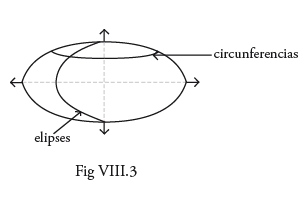
\includegraphics{./tex_imgs/repslatex-img48.png}
\end{marginfigure}
 

\ \ El eje fundamental del sistema de referencia es el eje de
rotación, el plano fundamental es el que es normal al eje de
revolución y pasa por el centro del elipsoide, corta al mismo en una
sección circular llamada ecuador elipsóidico, cuyo radio es el
semieje mayor de la elipse {\textquotedblleft}a{\textquotedblright}.

\begin{marginfigure}
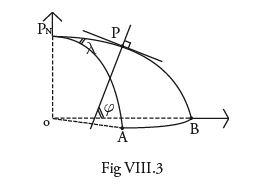
\includegraphics{./tex_imgs/repslatex-img49.png}
\end{marginfigure}
 

\ \ Dado un punto P cualquiera sobre el elipsoide, es posible trazar un
plano tangente a la superficie que contenga a P, la recta que pasa por
P y es perpendicular al plano tangente, se denomina
{\textquotedblleft}normal al elipsoide{\textquotedblright}.

\ \ La latitud elipsóidica  ${\varphi }$ o geodésica del punto P
sobre el elipsoide se define como el ángulo entre la normal en P y el
ecuador elipsóidico; se mide de 0 a 90{\textordmasculine}, positivo
al Norte y negativo al Sur.

\ \ La longitud elipsóidica  ${\lambda }$ o geodésica del punto P es
el ángulo diedro entre el meridiano que pasa por P y otro definido
como origen; se mide de 0 a 180{\textordmasculine}, positivo hacia el
este y negativo hacia el Oeste.

\ \ El acimut elipsóidico A es el ángulo entre dos planos, ambos
contienen a la normal al elipsoide en P: uno contiene a los polos y el
otro a la dirección considerada.

VIII.3.- CORTES NORMALES.

\begin{marginfigure}
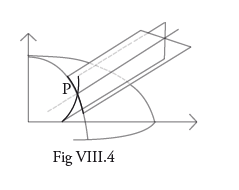
\includegraphics{./tex_imgs/repslatex-img50.png}
\end{marginfigure}
 

\ \ Dada una superficie cualquiera, se puede considerar en un punto P
sobre la misma un haz de infinitos planos que contienen a la normal a
la superficie en P. Dichos planos son llamados planos normales y
determinan \textbf{secciones normales}.
Las secciones normales al elipsoide son las que se obtienen de la
intersección de la superficie con los planos que contienen la normal
al elipsoide. Existen infinitas secciones normales en todo punto P del
elipsoide; todas son elipses en el caso del elipsoide de revolución.
Las secciones se caracterizan por acimut. Así habrá una sección
de acimut cero: llamada de sección meridiana, y otra de acimut de
90°: la sección normal al meridiano.

\subsection{Radios de Curvatura}

\ \ Los radios de curvatura que son de interés son los de las
secciones normales al elipsoide, y si existen infinitas secciones
normales hay infinitos radios de curvatura.

\begin{marginfigure}
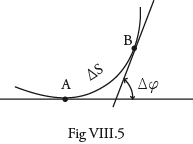
\includegraphics{./tex_imgs/repslatex-img51.png}
\end{marginfigure}
 

\ \ Dada una curva plana se define como curvatura media, al cociente
entre el ángulo que forman las tangentes a la curva en los puntos
extremos del arco y la longitud del arco; por lo tanto:

\begin{equation*}
{C_{{m}}=\frac{\mathit{\Delta \varphi }}{\mathit{\Delta S}}}
\end{equation*}

\begin{equation*}
\Delta S >> AB
\end{equation*}

Se llama curvatura en un punto A, al límite:

\begin{equation*}
  C = \lim_{\Delta S \to 0} \frac{\Delta \Phi}{\Delta S} = \frac{d \Phi}{dS}
\end{equation*}
 

En una circunferencia, la curvatura será:

\begin{equation*}
{\frac{\mathit{d\varphi
}}{\normalsubformula{\text{dS}}}=\frac{\mathit{d\varphi }}{R\cdot
\mathit{d\varphi }}}
\end{equation*}
\begin{equation*}
{C=\frac{1}{R}}
\end{equation*}
La curvatura es la inversa del radio. Se llama en general radio de
curvatura en un punto de una curva dada, al valor recíproco de la
curvatura dada en el punto; su valor está dado por:

\begin{equation*}
{R=\frac{\left(1+y'^{{2}}\right)^{{\frac{3}{2}}}}{y\text{{\textquotesingle}{\textquotesingle}}}=\frac{\left(1+\left(\frac{\normalsubformula{\text{dy}}}{\normalsubformula{\text{dx}}}\right)^{{2}}\right)^{{\frac{3}{2}}}}{\frac{d^{{2}}y}{\normalsubformula{\text{dx}}^{{2}}}}}
\end{equation*}

De los infinitos radios de curvatura de las secciones normales en un
punto del elipsoide, habrá uno de valor máximo y otro de valor
mínimo, llamados radios principales de curvatura, y son:

\ \ M: el radio de curvatura del meridiano o sección meridiana.
Corresponde a acimut cero, y es el menor.

\ \ N: el radio de curvatura de la sección normal al meridiano o
primer vertical. Corresponde a acimut de noventa grados y es el radio
mayor.

\begin{marginfigure}
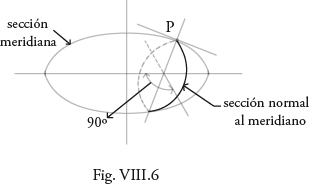
\includegraphics{./tex_imgs/repslatex-img54.png}
\end{marginfigure}
 

\ \ Estos radios de curvatura tienen un papel importante no solo en la
Geodesia,  sino además en la Cartografía, en las deducciones de las
expresiones de la proyección Gauss-Kruger, por lo tanto el
propósito es determinar los valores de M y N en función del
elipsoide, es decir se sus parámetros y de la posición del punto
sobre el mismo, es decir de sus coordenadas. 

\ \ Tanto M y N son función de los parámetros del elipsoide y de la
latitud solamente, ya que sus secciones meridianas son iguales.

\begin{marginfigure}
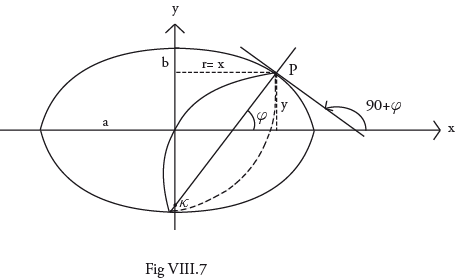
\includegraphics{./tex_imgs/repslatex-img55.png}
\end{marginfigure}
 

\ \ Se parte de la ecuación de la elipse meridiana y la del radio de
curvatura. En la elipse meridiana (Fig. VIII.7),
{\textquotedblleft}a{\textquotedblright} es el radio del ecuador y
{\textquotedblleft}b{\textquotedblright} el radio polar. Sea P un punto
cualquiera sobre la elipse meridiana, el ángulo que forma la normal
en P con el eje mayor es la latitud  ${\varphi }$. Trazando la tangente
en el punto P, ésta forma con el eje de las x el ángulo
(90{\textordmasculine}+ ${\varphi }$). Tanto x e y pueden considerarse
como funciones de una única variable  ${\varphi }$, que es la que
interesa en Geodesia y Cartografía. Se puede imaginar el punto P
moviéndose sobre la elipse desde el ecuador hasta el polo; la latitud
varía de 0 a 90{\textordmasculine}, x disminuye de
{\textquotedblleft}a{\textquotedblright} a cero, e y crece de cero a
{\textquotedblleft}b{\textquotedblright}. Si x e y son funciones de la
latitud, también lo son sus derivadas, las que expresadas en
función de la latitud se introducen en la ecuación del radio de
curvatura para encontrar M y N.

\ \ El radio de curvatura de la sección meridiana M es:

\begin{equation*}
{M=\frac{a^{{2}}\cdot b^{{2}}}{\left[a^{{2}}\cdot \text{cos}^{{2}}\left(\varphi \right)+b^{{2}}\cdot \normalsubformula{\text{sen}}^{{2}}\left(\varphi \right)\right]^{{\frac{3}{2}}}}}
\end{equation*}

se puede expresar también en función de la excentricidad:

\begin{equation*}
{M=\frac{a^{{2}}\cdot \left(1-e^{{2}}\right)}{\left[1-e^{{2}}\cdot \normalsubformula{\text{sen}}^{{2}}\left(\varphi \right)\right]^{{\frac{3}{2}}}}}
\end{equation*}

\ \ Para calcular el radio de curvatura de la sección normal al
meridiano, se establece la ecuación de la elipse correspondiente a
esa sección y se determina el radio de curvatura en el punto que
interesa, llegando a las siguientes expresiones:

\begin{equation*}
{N=\frac{a}{\left[1-e^{{2}}\cdot \normalsubformula{\text{sen}}^{{2}}\left(\varphi \right)\right]^{{\frac{1}{2}}}}}
\end{equation*}

\begin{equation*}
{N=\frac{a^{{2}}}{\left[a^{{2}}\cdot \text{cos}^{{2}}\left(\varphi \right)+b^{{2}}\cdot \normalsubformula{\text{sen}}^{{2}}\left(\varphi \right)\right]^{{\frac{1}{2}}}}}
\end{equation*}

\ \ Se demuestra además que el radio de un paralelo cualquiera de
latitud  ${\varphi }$; ver fig VIII.7:

\begin{equation*}
{r=N\cdot \text{cos}\left(\varphi \right)}
\end{equation*}
Por lo tanto:

\begin{equation*}
{N=\frac{r}{\text{cos}\left(\varphi \right)}}
\end{equation*}
de donde N es el segmento PK de la Figura VIII.7.

\ \ Para algunas deducciones puede ser necesario que los radios de
curvatura se expresen en función de la segunda excentricidad; se
determina que:

\begin{equation*}
{M=\frac{a^{{2}}}{b\cdot \left[1+e'^{{2}}\cdot \text{cos}^{{2}}\left(\varphi \right)\right]^{{\frac{3}{2}}}}}
\end{equation*}

\begin{equation*}
{N=\frac{a^{{2}}}{b\cdot \left[1+e'^{{2}}\cdot \text{cos}^{{2}}\left(\varphi \right)\right]^{{\frac{1}{2}}}}}
\end{equation*}

Los valores en el polo se encuentran haciéndolo  ${\varphi =\text{90}}$ y se obtiene:

\begin{equation*}
{M=N=\frac{a^{{2}}}{b}}
\end{equation*}
En el ecuador  ${\varphi =0}$, se tiene que:

\begin{equation*}
{M=a\cdot \left(1-e^{{2}}\right)}
\end{equation*}
\begin{equation*}
{N=a}
\end{equation*}
donde M es menor que N; se evidencia que N es siempre mayor que M,
llegándose a igualar en el polo.

\ \ Se deduce también que el radio de curvatura de una sección
normal de acimut cualquiera es igual a:

\begin{equation*}
{R_{{A}}=\frac{M\cdot N}{M\cdot \normalsubformula{\text{sen}}^{{2}}\left(A\right)+N\cdot \text{cos}^{{2}}\left(A\right)}}
\end{equation*}

\ \ En muchas aplicaciones geodésicas y cartográficas, es
suficientemente aproximado utilizar una esfera auxiliar que reemplaza
al elipsoide, cuya superficie se adapta lo mejor posible en las
proximidades del punto de interés.

\ \ Esta esfera tiene un radio, que es el valor medio de todos los
radios de curvatura del elipsoide en un punto; esto es:

\begin{equation*}
{R=\frac{1}{\left(\wideslash{\pi }{2}\right)}\cdot \overset{{A=\wideslash{\pi }{2}}}{\underset{{A=0}}{\int }}{R_{{A}}\cdot \normalsubformula{\text{dA}}}}
\end{equation*}
Se demuestra que el radio de la esfera que mejor se adapta es:

\begin{equation*}
{R=\sqrt{M\cdot N}}
\end{equation*}

VIII.5.- ARCO DE MERIDIANO ELIPSÓIDICO.

\begin{marginfigure}
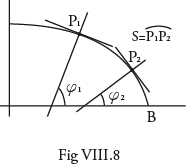
\includegraphics{./tex_imgs/repslatex-img56.png}
\end{marginfigure}
 

\ \ Si se desea calcular la longitud la longitud de un arco de meridiano
entre dos puntos P1 y P2, teniendo en cuenta que un diferencial de arco
está dado por:

\begin{equation*}
{\normalsubformula{\text{dS}}=M\cdot \mathit{d\varphi }}
\end{equation*}
Se debe integrar dicho elemento entre los valores de  ${\varphi _{{1}}}$
y  ${\varphi _{{2}}}$; esto es:

\begin{equation*}
{S=\overset{\varphi _{{2}}}{\underset{{\varphi _{{1}}}}{\int }}{M\cdot
\mathit{d\varphi }}}
\end{equation*}

\begin{equation*}
{S=\overset{\varphi _{{2}}}{\underset{{\varphi _{{1}}}}{\int}}{\frac{a\cdot \left(1-e^{{2}}\right)}{\left[1-e^{{2}}\cdot \normalsubformula{\text{sen}}^{{2}}\left(\varphi \right)\right]^{{\frac{3}{2}}}}\cdot \mathit{d\varphi }}}
\end{equation*}

\begin{equation*}
{S=a\cdot \left(1-e^{{2}}\right)\cdot \overset{\varphi _{{2}}}{\underset{{\varphi _{{1}}}}{\int }}{\frac{\mathit{d\varphi}}{\left[1-e^{{2}}\cdot \normalsubformula{\text{sen}}^{{2}}\left(\varphi \right)\right]^{{\frac{3}{2}}}}}}
\end{equation*}

Esta integral se resuelve mediante el desarrollo de la serie binomial
del integrando:

\begin{equation*}
\begin{matrix}{\left[1-e^{{2}}\cdot \normalsubformula{\text{sen}}^{{2}}\left(\varphi \right)\right]^{{-{\frac{3}{2}}}}=1+\frac{3}{2}\cdot e^{{2}}\cdot \normalsubformula{\text{sen}}^{{2}}\left(\varphi \right)+\frac{3}{2}\cdot {\frac{5}{4}}\cdot e^{{4}}\cdot \normalsubformula{\text{sen}}^{{4}}\left(\varphi \right)+\frac{3}{2}\cdot {\frac{5}{4}}\cdot {\frac{7}{6}}\cdot e^{{6}}\cdot \normalsubformula{\text{sen}}^{{6}}\left(\varphi \right)}\hfill\null \\+{\frac{3}{2}}\cdot {\frac{5}{4}}\cdot {\frac{7}{6}}\cdot {\frac{9}{8}}\text{.}\text{.}\text{.}\text{.}\text{.}\text{.}\text{.}\text{.}\text{.}\text{.}\text{.}\text{.}\text{.}\text{.}\text{.}\text{.}\text{.}\text{.}\text{.}\hfill\null \end{matrix}\hfill 
\end{equation*}

la cual se debe multiplicar por  ${\mathit{d\varphi }}$ y ejecutar la
integración término por término, pero antes de proceder a la
interpretación, se reemplazan las potencias del seno de la latitud en
funciones trigonométricas múltiplos de  ${\varphi }$, como se
indica a continuación:

\begin{equation*}
{\normalsubformula{\text{sen}}^{{2}}\left(\varphi
\right)=\frac{1}{2}-\frac{1}{2}\cdot \text{cos}^{{2}}\left(\varphi
\right)}
\end{equation*}
\begin{equation*}
{\normalsubformula{\text{sen}}^{{4}}\left(\varphi
\right)=\frac{3}{8}-\frac{1}{2}\cdot \text{cos}^{{2}}\left(\varphi
\right)+\frac{1}{8}\cdot \text{cos}^{{4}}\left(\varphi \right)}
\end{equation*}
\begin{equation*}
{\normalsubformula{\text{sen}}^{{6}}\left(\varphi
\right)=\frac{5}{\text{16}}-\frac{\text{15}}{\text{32}}\cdot
\text{cos}^{{2}}\left(\varphi \right)+\frac{3}{\text{16}}\cdot
\text{cos}^{{4}}\left(\varphi \right)-\frac{1}{\text{32}}\cdot
\text{cos}^{{6}}\left(\varphi \right)}
\end{equation*}
\begin{equation*}
{\normalsubformula{\text{sen}}^{{8}}\left(\varphi
\right)=\frac{\text{35}}{\text{128}}-\frac{7}{\text{16}}\cdot
\text{cos}^{{2}}\left(\varphi \right)+\frac{7}{\text{32}}\cdot
\text{cos}^{{4}}\left(\varphi \right)-\frac{1}{\text{16}}\cdot
\text{cos}^{{6}}\left(\varphi \right)+\frac{1}{\text{128}}\cdot
\text{cos}^{{8}}\left(\varphi \right)}
\end{equation*}
Estos últimos valores se reemplazan en la (VIII.10), y quedan
multiplicados por los factores  ${\frac{3}{2}\cdot e^{{2}}}$, 
${\frac{3}{2}\cdot {\frac{5}{4}}\cdot e^{{4}}}$, etc. Se agrupan luego
según los cosenos múltiplos de la latitud, y para abreviar conviene
escribir:

\begin{equation*}
{A=1+\frac{3}{4}\cdot
e^{{2}}+\frac{\text{45}}{\text{64}}e^{{4}}+\frac{\text{175}}{\text{256}}\cdot
e^{{6}}+\frac{\text{11025}}{\text{16384}}\cdot
e^{{8}}\text{.}\text{.}\text{.}\text{.}\text{.}\text{.}\text{.}\text{.}\text{.}\text{.}\text{.}\text{.}\text{.}}
\end{equation*}

\begin{equation*}
{B=-\left[\frac{3}{4}\cdot
e^{{2}}+\frac{\text{15}}{\text{16}}e^{{4}}+\frac{\text{525}}{\text{512}}\cdot
e^{{6}}+\frac{\text{2205}}{\text{2048}}\cdot
e^{{8}}+\text{.}\text{.}\text{.}\text{.}\text{.}\text{.}\text{.}\text{.}\text{.}\text{.}\text{.}\text{.}\text{.}\right]}
\end{equation*}

\begin{equation*}
{C=\overset{}{{}}\overset{}{{}}\overset{}{{}}\overset{}{{}}\overset{}{{}}\left[\frac{\text{15}}{\text{64}}e^{{4}}+\frac{\text{105}}{\text{256}}\cdot e^{{6}}+\frac{\text{2205}}{\text{4096}}\cdot e^{{8}}+\text{.}\text{.}\text{.}\text{.}\text{.}\text{.}\text{.}\text{.}\text{.}\text{.}\text{.}\text{.}\text{.}\right]}
\end{equation*}

\begin{equation*}
{D=\overset{}{{}}\overset{}{{}}\overset{}{{}}\overset{}{{}}\overset{}{{}}\overset{}{{}}\overset{}{{}}\overset{}{{}}\overset{}{{}}-\left[\frac{\text{35}}{\text{512}}\cdot
e^{{6}}+\frac{\text{315}}{\text{2048}}\cdot
e^{{8}}+\text{.}\text{.}\text{.}\text{.}\text{.}\text{.}\text{.}\text{.}\text{.}\text{.}\text{.}\text{.}\text{.}\right]}
\end{equation*}

\begin{equation*}
{E=\overset{}{{}}\overset{}{{}}\overset{}{{}}\overset{}{{}}\overset{}{{}}\overset{}{{}}\overset{}{{}}\overset{}{{}}\overset{}{{}}\overset{}{{}}\overset{}{{}}\overset{}{{}}\overset{}{{}}\overset{}{{}}\overset{}{{}}+\left[\frac{\text{315}}{\text{16384}}\cdot
e^{{8}}+\text{.}\text{.}\text{.}\text{.}\text{.}\text{.}\text{.}\text{.}\text{.}\text{.}\text{.}\text{.}\text{.}\right]}
\end{equation*}

Reemplazando en (VIII.10) se tiene que:

\begin{equation*}
{\left[1-e^{{2}}\cdot \normalsubformula{\text{sen}}^{{2}}\left(\varphi
\right)\right]^{{\frac{-3}{2}}}=A+B\cdot \text{cos}\left(2\varphi
\right)+C\cdot \text{cos}\left(4\varphi \right)+D\cdot
\text{cos}\left(6\varphi \right)+E\cdot \text{cos}\left(8\varphi
\right)+\text{.}\text{.}\text{.}\text{.}}
\end{equation*}

Multiplicando por  ${a\cdot \left(1-e^{{2}}\right)\cdot \mathit{d\varphi}}$,
y teniendo en cuenta la (VIII.9), se tiene que:

\begin{equation*}
{S=a\cdot \left(1-e^{{2}}\right)\overset{\varphi
_{{2}}}{\underset{{\varphi _{{1}}}}{\int }}{\left[A+B\cdot
\text{cos}\left(2\varphi \right)+C\cdot \text{cos}\left(4\varphi
\right)+D\cdot \text{cos}\left(6\varphi \right)+E\cdot
\text{cos}\left(8\varphi
\right)+\text{.}\text{.}\text{.}\text{.}\right]}{?\mathit{d\varphi }}}
\end{equation*}

Integrando esta última expresión se obtiene el arco de meridiano
elipsóidico entre dos valores de latitud dados; por lo tanto:

\begin{equation*}
{S=a\cdot \left(1-e^{{2}}\right)\cdot \left(A+\frac{B}{2}\cdot
\normalsubformula{\text{sen}}\left(2\varphi \right)+\frac{C}{4}\cdot
\normalsubformula{\text{sen}}\left(4\varphi \right)+\frac{D}{6}\cdot
\normalsubformula{\text{sen}}\left(6\varphi \right)+\frac{E}{8}\cdot
\normalsubformula{\text{sen}}\left(8\varphi
\right)+\text{.}\text{.}\text{.}\text{.}\right)|_{{\varphi
_{{1}}}}^{\varphi _{{2}}}}
\end{equation*}

En esta expresión el valor de la latitud que acompa\~na a A se debe
introducir en radianes.

En caso que se desee introducir la latitud en grados sexagesimales, hay
que agregar en el primer término del paréntesis el factor 
${\frac{1}{\rho _{{o}}}}$, siendo el  ${\rho _{{o}}}$ el número de
grados contenidos en un radián.

Para simplificar aún más la última expresión, se puede escribir:

\begin{equation*}
{\alpha =a\cdot \left(1-e^{{2}}\right)\cdot A}
\end{equation*}

\begin{equation*}
{\beta =\frac{a}{2}\cdot \left(1-e^{{2}}\right)\cdot B}
\end{equation*}

\begin{equation*}
{\gamma =\frac{a}{4}\cdot \left(1-e^{{2}}\right)\cdot C}
\end{equation*}

\begin{equation*}
{\delta =\frac{a}{6}\cdot \left(1-e^{{2}}\right)\cdot D}
\end{equation*}

\begin{equation*}
{\varepsilon =\frac{a}{8}\cdot \left(1-e^{{2}}\right)\cdot E}
\end{equation*}

con lo cual la expresión del arco se transforma en:

\begin{equation*}
S=\alpha \varphi + \beta sen (2\varphi) + \gamma sen (4\phi) + \delta sen (6\varphi) + \epsilon sen (8\varphi) + ... |_{\Phi1}^{\Phi2}
\end{equation*}
%   (VIII.11)
\
\ \ Por medio de las expresiones vistas se calculan de una vez, para un
determinado elipsoide, las constantes  ${\alpha ,\beta ,\gamma ,\delta
,\varepsilon }$, las que dependen únicamente del semieje mayor y de
la excentricidad de la elipse meridiana. Luego con la expresión
(VIII.11) se puede calcular un arco de meridiano entre dos valores de
latitud cualesquiera.

\ \ En Cartografía existen dos arcos de meridiano de especial
interés, como se verá más adelante. Éstos son el arco de
meridiano desde el ecuador hasta un punto de latitud cualquiera y el
arco de meridiano desde el polo sur al punto de la latitud considerada,
valores éstos que forman parte de las expresiones de las coordenadas
de U.T.M. y Gauss-Kruger, respectivamente. 

\ \ En el primer caso, \(\varphi_1=0\) , la expresión %(VIII.11)
se transforma en:

 \begin{equation*}
S=\alpha \varphi + \beta sen (2\varphi) + \gamma sen (4\phi) + \delta sen (6\varphi) + \epsilon sen (8\varphi)
\end{equation*}
%   (VIII.12)

 En el segundo \(\varphi_1=90°=\frac{\varpi}{2}\), se tiene que la %(VIII.11)
 se transforma en:

 \begin{equation*}
S=\alpha \left( \varphi + \frac{\varpi}{2} \right) + \beta sen (2\varphi) + \gamma sen (4\phi) + \delta sen (6\varphi) + \epsilon sen (8\varphi)
\end{equation*}
%   (VIII.13)

recordando que el valor de la latitud en el primer término debe
expresarse en radianes.

VIII.6.- ARCO DE PARALELO ELIPSÓIDICO.

\begin{marginfigure}
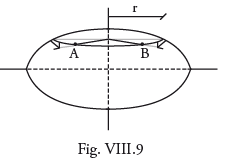
\includegraphics{./tex_imgs/repslatex-img64.png}
\end{marginfigure}
 

Dado que el elipsoide es de revolución, los paralelos son
circunferencias. Un elemento de arco de paralelo está dado por:

\[
dp=r\,d\lambda=N\,cos(\varphi)\,d\lambda
\]

El valor de un arco de paralelo entre las longitudes \(\lambda_1\)
  y \(\lambda_2\) está dado por:

  \[
  AB=N\,cos(\varphi)\,(\lambda_2-\lambda_1)
  \]

IX.1.- MÓDULO DE DEFORMACIÓN LINEAL

Siguiendo la misma secuencia teórica del capítulo IV, se desarrollan
las expresiones del módulo de deformación lineal, pero considerando
como figura de la tierra el elipsoide.

\begin{marginfigure}
\includegraphics{./tex_imgs/repslatex-img77.png}
\end{marginfigure}
 

\ \ Sean dos puntos sobre el elipsoide, P y Q, de coordenadas 
${P(\varphi ,\lambda )}$ y  ${Q(\varphi +\mathit{d\varphi },\lambda
+\mathit{d\lambda })}$. Los arcos de paralelo y meridiano elementales
son respectivamente: 

\begin{equation*}
{\mathit{d\rho }=N\cdot \text{cos}\left(\varphi \right)\cdot
\mathit{d\lambda }}
\end{equation*}
\begin{equation*}
{\normalsubformula{\text{dm}}=M\cdot \mathit{d\varphi }}
\end{equation*}
De donde la distancia elemental es:

 ${\normalsubformula{\text{dL}}=\sqrt{\left(M\cdot \mathit{d\varphi
}\right)^{{2}}+\left[N\cdot \text{cos}\left(\varphi \right)\cdot
\mathit{d\lambda }\right]^{{2}}}}$  (IX.1)

El área del rectángulo individual es igual:

\ \  ${\normalsubformula{\text{dS}}=M\cdot N\cdot
\text{cos}\left(\varphi \right)\cdot \mathit{d\varphi }\cdot
\mathit{d\lambda }}$  (IX.2)

Y el acimut del elemento distancia dL es:

\ \  ${\normalsubformula{\text{tg}}\left(A\right)=\frac{N\cdot
\text{cos}\left(\varphi \right)\cdot \mathit{d\lambda }}{M\cdot
\mathit{d\varphi }}}$  (IX.3)

Las expresiones de las imágenes de dL, dS y A en el plano son las
mismas vistas en (IV.1).

Por lo tanto el módulo de deformación es:

\begin{equation*}
{m_{{l}}=\frac{\normalsubformula{\text{dl}}}{\normalsubformula{\text{dL}}}}
\end{equation*}
Reemplazando en la (IV.5) y la (IX.1) se tiene:

\begin{equation*}
{m_{{l}}^{{2}}=\frac{\left(\normalsubformula{\text{dx}}\right)^{{2}}+\left(\normalsubformula{\text{dy}}\right)^{{2}}}{\left(M\cdot
\mathit{d\varphi }\right)^{{2}}+\left[N\cdot \text{cos}\left(\varphi
\right)\cdot \mathit{d\lambda }\right]^{{2}}}}
\end{equation*}
De la misma manera que se dedujo en la (IV.26):

\begin{equation*}
{m_{{l}}^{{2}}=\frac{E\cdot \left(\mathit{d\varphi }\right)^{{2}}+G\cdot
\left(\mathit{d\lambda }\right)^{{2}}+2\cdot F\cdot \mathit{d\varphi
}\cdot \mathit{d\lambda }}{\left(M\cdot \mathit{d\varphi
}\right)^{{2}}+\left[N\cdot \text{cos}\left(\varphi \right)\cdot
\mathit{d\lambda }\right]^{{2}}}}
\end{equation*}
Siendo el mismo razonamiento que en (IV.27)

\ \  ${m_{{l}}^{{2}}=\frac{E}{M^{{2}}}\cdot
\text{cos}^{{2}}\left(A\right)+G\cdot
{\frac{\normalsubformula{\text{sen}}^{{2}}\left(A\right)}{\left[N\cdot
\text{cos}\left(\varphi \right)\right]^{{2}}}}+F\cdot
{\frac{\normalsubformula{\text{sen}}\left(2A\right)}{M\cdot N\cdot
\text{cos}\left(\varphi \right)}}}$  (IX.4)

De esta última expresión se desprende que el módulo de
deformación lineal es en elipsoide es función de la latitud y del
acimut, y por supuesto de la ley de representación.

\ \ Para hallar el máximo y mínimo de la expresión (IX.4) se
diferencia el módulo de deformación lineal en función del acimut,
y se iguala la derivada a cero, como se efectuó en (IV.28); en este
caso se arriba a la siguiente expresión:

\ \  ${\normalsubformula{\text{tg}}\left(2A\right)=\frac{2\cdot F\cdot
M\cdot N\cdot \text{cos}\left(\varphi \right)}{\left[E\cdot N\cdot
\text{cos}\left(\varphi \right)-G\cdot M\right]}}$  (IX.5)

\ \ Para encontrar las expresiones de los módulos de deformación
lineal según los meridianos y según los paralelos, se debe hacer en
la (IX.4) A=0 y A=90, respectivamente y se obtiene:

\begin{equation*}
{m_{{l}}^{{m}}=\frac{\sqrt{E}}{M}}
\end{equation*}
 (IX.6)

\begin{equation*}
{m_{{l}}^{{p}}=\frac{\sqrt{C}}{N\cdot \text{cos}\left(\varphi \right)}}
\end{equation*}
\ \ A continuación se desarrollarán las proyecciones geodésicas de
mayor uso en la práctica: estereográfica polar, Mercator y Cónica
de Lambert.

\ \ En capítulo aparte las proyecciones Gauss-Kruger, y su
aplicación en la Argentina y la proyección U.T.M. (Universal
Transversal Mercator) serán desarrolladas, por lo particular de su
planteo y por la amplia difusión de ambas proyecciones en todo el
mundo.

X.2.- PROYECCIÓN GAUSS-KR\"UGER.

\ \ Dados dos puntos sobre el elipsoide infinitamente próximos (figura
IX.2), ambos vienen caracterizados por sus coordenadas geográficas
latitud y longitud. Teniendo en cuenta que ambos puntos son
infinitamente próximos, se puede considerar que la parcela
elipsóidica que abarcan no tienen curvatura, es decir que es un plano
que se denominará {\textquotedblleft}z{\textquotedblright}, es decir
que la superficie elemental  ${\left(\mathit{d\varphi
},\mathit{d\lambda }\right)}$ se supone plana.

\ \ Ambos puntos tienen su imagen plana, cuyas posiciones se
caracterizan por sus coordenadas planas ortogonales X e Y en la carta,
que se denominará plano de las
{\textquotedblleft}u{\textquotedblright}.

Se trata de establecer la relación funcional entre la superficie
elipsóidica elemental con la correspondiente superficie plana, con la
condición que la representación sea conforme. De acuerdo con lo
anteriormente expuesto se hace uso de la funciones de variable compleja
porque ellas satisfacen dicha condición.

\ \ Se forman para cada plano las variables complejas:

\begin{equation*}
{z=\varphi +\mathit{i\lambda }}
\end{equation*}
\begin{equation*}
{u=X+\normalsubformula{\text{iY}}}
\end{equation*}
Ambas variables están ligadas por la función de variable compleja:

 ${u=f\left(z\right)}$

O sea:

\ \  ${X+\normalsubformula{\text{iY}}=f\left(\varphi +\mathit{i\lambda
}\right)}$  (X.7)

Formando la variable compleja  ${\varphi +\mathit{i\lambda }}$ no se ha
elegido la misma unidad lineal para la parte real y la parte imaginaria
de la variable. Si se incrementan en
1{\textquoteright}{\textquoteright} por ejemplo la latitud y longitud,
el arco de meridiano es siempre el mismo para cualquier latitud, no
así el arco de paralelo que disminuye a medida que la longitud
aumenta.

\ \ Los arcos de meridiano y paralelo en el elipsoide son
respectivamente:

\begin{equation*}
{\normalsubformula{\text{dm}}=M\cdot \mathit{d\varphi }}
\end{equation*}
\begin{equation*}
{\normalsubformula{\text{dp}}=N\cdot \text{cos}\left(\varphi
\right)\cdot \mathit{d\lambda }}
\end{equation*}
En la esfera:

\begin{equation*}
{\normalsubformula{\text{dm}}=R\cdot \mathit{d\varphi }}
\end{equation*}
\begin{equation*}
{\normalsubformula{\text{dp}}=R\cdot \text{cos}\left(\varphi
\right)\cdot \mathit{d\lambda }}
\end{equation*}
Por lo tanto el arco de paralelo disminuye de acuerdo con el coseno de
la latitud. Por ejemplo 1{\textquoteright}{\textquoteright} en el
ecuador y a 60{\textdegree} de latitud le corresponden los siguientes
arcos de meridiano y paralelo:


${\normalsubformula{\text{dm}}\left(0{}^{\circ}\right)=\text{30}m}$\ \ \ \ 
  ${\normalsubformula{\text{dp}}\left(0{}^{\circ}\right)=\text{30}m}$


${\normalsubformula{\text{dm}}\left(\text{60}{}^{\circ}\right)=\text{30}m}$\ \ \ \ 
 
${\normalsubformula{\text{dp}}\left(\text{50}{}^{\circ}\right)=\text{15}m}$

\ \ Es decir, que sobre la superficie elipsóidica considerada plana,
no se tienen cuadrados elementales sino rectángulos elementales, por
no producir el mismo incremento lineal sobre el elipsoide, incrementos
iguales en latitud y longitud. Si:

\begin{equation*}
{\mathit{d\varphi }=\mathit{d\lambda }}
\end{equation*}
Las unidades lineales en el sentido de la latitud y la longitud están
en la relación:

\begin{equation*}
{\frac{\normalsubformula{\text{dp}}}{\normalsubformula{\text{dm}}}=\frac{M}{N\cdot
\text{cos}\left(\varphi \right)}}
\end{equation*}
\ \ Para igualar los arcos de meridiano y paralelo se sustituye la
latitud {\textquotedblleft} ${\varphi }${\textquotedblright} por una
nueva variable {\textquotedblleft}q{\textquotedblright} llamada latitud
isométrica, contada también a partir del ecuador de manera que el
elemento de meridiano se exprese:

\begin{equation*}
{M\cdot \mathit{d\varphi }=N\cdot \text{cos}\left(\varphi \right)\cdot
\normalsubformula{\text{dq}}}
\end{equation*}
Porque se desea que para iguales incrementos de latitud isométrica y
longitud:

\begin{equation*}
{\normalsubformula{\text{dq}}=\mathit{d\lambda }}
\end{equation*}
Se produzcan iguales incrementos lineales sobre meridianos y paralelos.
Por lo tanto:

 ${\normalsubformula{\text{dq}}=\frac{M\cdot \mathit{d\varphi }}{N\cdot
\text{cos}\left(\varphi \right)}}$  (X.8)

En el caso de una esfera sonde M=N=R se tiene que:

\ \  ${\normalsubformula{\text{dq}}=\frac{\mathit{d\varphi
}}{\text{cos}\left(\varphi \right)}}$  (X.8{\textquoteright})

Si por ejemplo  ${\normalsubformula{\text{dq}}=\mathit{d\lambda
}=1\text{{\textquotesingle}{\textquotesingle}}}$, en la latitud de
60{\textdegree} se tiene que:

\begin{equation*}
{\normalsubformula{\text{dm}}=R\cdot \mathit{d\varphi }=R\cdot
\text{cos}\left(\varphi \right)\cdot
\normalsubformula{\text{dq}}=\text{15}m}
\end{equation*}
\begin{equation*}
{\normalsubformula{\text{dm}}=R\cdot \mathit{d\varphi }=R\cdot
\text{cos}\left(\varphi \right)\cdot
\normalsubformula{\text{dq}}=\text{15}m}
\end{equation*}
Integrando las (X.8) y (X.8{\textquoteright}):

\begin{equation*}
{q=\text{ln}\left[\normalsubformula{\text{tg}}\left(\text{45}\text{{\textdegree}+}\frac{\varphi
}{2}\right)\right]-\frac{e}{2}\cdot \text{ln}\left(\frac{1-e\cdot
\normalsubformula{\text{sen}}\left(\varphi \right)}{1+e\cdot
\normalsubformula{\text{sen}}\left(\varphi \right)}\right)}
\end{equation*}
\begin{equation*}
{q=\text{ln}\left[\normalsubformula{\text{tg}}\left(\text{45}\text{{\textdegree}+}\frac{\varphi
}{2}\right)\right]-\frac{e}{2}\cdot \text{ln}\left(\frac{1-e\cdot
\normalsubformula{\text{sen}}\left(\varphi \right)}{1+e\cdot
\normalsubformula{\text{sen}}\left(\varphi \right)}\right)}
\end{equation*}

\end{document}
